\documentclass{chi-ext}
% Please be sure that you have the dependencies (i.e., additional LaTeX packages) to compile this example.
% See http://personales.upv.es/luileito/chiext/

%% EXAMPLE BEGIN -- HOW TO OVERRIDE THE DEFAULT COPYRIGHT STRIP -- (July 22, 2013 - Paul Baumann)
% \copyrightinfo{Permission to make digital or hard copies of all or part of this work for personal or classroom use is granted without fee provided that copies are not made or distributed for profit or commercial advantage and that copies bear this notice and the full citation on the first page. Copyrights for components of this work owned by others than ACM must be honored. Abstracting with credit is permitted. To copy otherwise, or republish, to post on servers or to redistribute to lists, requires prior specific permission and/or a fee. Request permissions from permissions@acm.org. \\
% {\emph{IHM14}}, 28-31 Octobre, 2014, Lille, France. \\
% Copyright \copyright~2014 ACM ISBN/14/04...\$15.00. \\
% DOI string from ACM form confirmation}
%% EXAMPLE END -- HOW TO OVERRIDE THE DEFAULT COPYRIGHT STRIP -- (July 22, 2013 - Paul Baumann)

\title{Test of Adaptable User Interfaces}

\numberofauthors{4}
% Notice how author names are alternately typesetted to appear ordered in 2-column format;
% i.e., the first 4 autors on the first column and the other 4 auhors on the second column.
% Actually, it's up to you to strictly adhere to this author notation.
\author{
  \alignauthor{
  	\textbf{Nelson}\\
  	\affaddr{AuthorCo, Inc.}\\
  	\affaddr{123 Author Ave.}\\
  	\affaddr{Authortown, PA 54321 USA}\\
  	\email{author1@anotherco.com}
  }\alignauthor{
  	\textbf{Julien}\\
  	\affaddr{AuthorCo, Inc.}\\
  	\affaddr{123 Author Ave.}\\
  	\affaddr{Authortown, PA 54321 USA}\\
  	\email{author5@anotherco.com}
  }
  \vfil
  \alignauthor{
  	\textbf{Lydie}\\
  	\affaddr{AuthorCo, Inc.}\\
  	\affaddr{123 Author Ave.}\\
  	\affaddr{Authortown, PA 54321 USA}\\
  	\email{author2@anotherco.com}
  }\alignauthor{
  	\textbf{Sophie}\\
  	\affaddr{AuthorCo, Inc.}\\
  	\affaddr{123 Author Ave.}\\
  	\affaddr{Authortown, PA 54321 USA}\\
  	\email{author6@anotherco.com}
  }
}

% Paper metadata (use plain text, for PDF inclusion and later re-using, if desired)
\def\plaintitle{Test of Adaptable User Interfaces}
\def\plainauthor{Nelson Mariano Leite Neto}
\def\plainkeywords{Guides, instructions, author's kit, conference publications}
\def\plaingeneralterms{Documentation, Standardization}

\hypersetup{
  % Your metadata go here
  pdftitle={\plaintitle},
  pdfauthor={\plainauthor},  
  pdfkeywords={\plainkeywords},
  pdfsubject={\plaingeneralterms},
  % Quick access to color overriding:
  %citecolor=black,
  %linkcolor=black,
  %menucolor=black,
  %urlcolor=black,
}

\usepackage{graphicx}   % for EPS use the graphics package instead
\usepackage{balance}    % useful for balancing the last columns
\usepackage{bibspacing} % save vertical space in references
%\usepackage{hyperref}
%\hypersetup{colorlinks=false}

%\widowpenalty=10000
%\clubpenalty=10000

\usepackage{epstopdf}

\begin{document}

\maketitle

\begin{abstract}
TODO - Lorem ipsum sed ut perspiciatis unde omnis iste natus error sit voluptatem accusantium doloremque laudantium, totam rem aperiam, eaque ipsa quae ab illo inventore veritatis et quasi architecto beatae vitae dicta sunt explicabo. Nemo enim ipsam voluptatem quia voluptas sit aspernatur aut odit aut fugit, sed quia consequuntur magni dolores eos qui ratione voluptatem sequi nesciunt. Neque porro quisquam est, qui dolorem ipsum quia dolor sit amet, consectetur, adipisci velit, sed quia non numquam eius modi tempora incidunt ut labore et dolore magnam aliquam quaerat voluptatem.
\end{abstract}

\keywords{\plainkeywords}
\textcolor{red}{Champs requis dans la version finale}

\category{H.5.m}{Information interfaces and presentation (e.g., HCI)}{Miscellaneous}. 
%See \cite{ACMCCS} 
Voir : \url{http://www.acm.org/about/class/1998/} 
pour une description du ACM Classification system.
\textcolor{red}{Champs requis dans la version finale}

\terms{\plaingeneralterms}
\textcolor{red}{Champs requis dans la version finale}


% =============================================================================
\section{Introduction}
% =============================================================================
Nowadays, with the rise of mobile devices such as notebooks, smartphones, smartwatches and tablets, there is computer systems running everywhere and in different \textit{contexts of use}, which involves three factors: the \textit{platform}, \textit{environment} and \textit{the user}~\cite{ui-eric-plasticity-vs-responsive}. These factors affect the interaction between the user and the system. This interaction happens through the \textit{user interface} (UI), and users have to deal with different UIs adapted to several contexts. Hence the term \textit{adaptable user interfaces}. All this allows to see that today developing UIs can be as complex as developing the core of the system. There are several questions to be considered, among them: quality. \textit{Software Testing} is one of the most used ways in the industry to assure quality~\cite{test-hdr-lydie}. It can be defined as a process, or a series of processes, designed to ensure computer code does what it was designed to do and, conversely, that it does not anything unintended~\cite{test-art-of-testing}. What is the impact of adaptable user interfaces on software testing? Are there already tools to test these adaptable UIs?

Answering these questions motivates the development of this project. In this work, we focus on the scenario of having different UIs for the same system. These UIs can be adapted to different devices or have different versions for the same device. For instance, we used as case study a smart home energy management system prototype with four equivalent versions: three for web and one for mobile environment. This exposes the problem which we focus: the repetitive work of writing and maintaining test scripts for different versions of the UIs of the same system.

Our contribution is the approach of automatically generate test scripts for each version of the UI of the same system from scripts written in a higher-level language. In other words, testers would be able to write test cases for all the versions using abstract descriptions. A tool would be responsible for interpreting these descriptions and generating test scripts ready to be executed for each version of the UI.

This paper is structured as follows. First, the related work is presented, explaining several concepts about test automation, UI testing and tools. Then, we explain the case study used in this research. Next, we show how test scripts can be generated from abstract descriptions using an existing tool. Finally, the conclusions that summarize our current results and proposed perspectives.

% =============================================================================
\section{Related Work}
% =============================================================================
With the popularity of Continuous Integration (CI), a software engineering practice in which isolated changes are immediately tested and reported on when they are added to a larger code base, the need of test automation has increased. Test automation can be achieved by three ways: the generation of test scripts, their execution and the analysis of the results. The scientific community has developed several approaches and tools for automation of regular and UI testing. Some of them will be presented below.

An example of automation for the generation of test scripts is Tobias~\cite{tobias}, a combinatorial tool that instantiates a large set of test sequences from an abstract description. Combinatorial testing allows to express a large set of test cases in a few lines. Tobias receives the abstract test and generates an executable test code containing several possible combinations of execution, according to the specification of the abstract code given. 

In the case of execution automation, several tools have been developed focusing on UI testing. There are tools that drive the UI as users do, triggering actions, navigating the system and checking the UI content. For instance, tools for web~\cite{watir, cucumber} and mobile~\cite{appium, selendroid} environments are responsible for interacting with the UI according to the scripts written by the testers. Besides, there are tools~\cite{selenium, monkeytalk} that are also able to generate test scripts, through the process of record and playback. The user interacts with the system, the tool records the actions, thus generating a test script that can be used thereafter for execution automation.

\marginpar{
\begin{figure}
  \begin{center}
  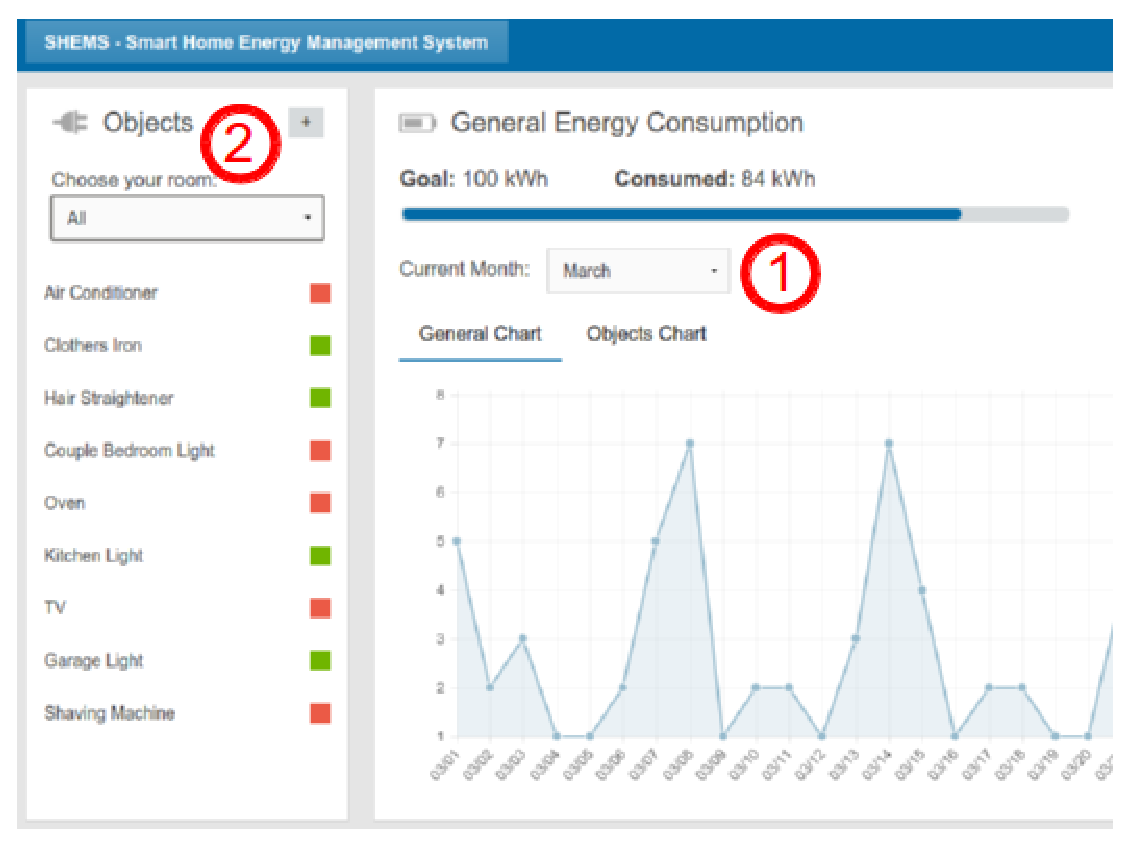
\includegraphics[width=\marginparwidth]{images/web0_goal-filter.eps}
  \caption{Web version. Number 1 represents the \textbf{goal} feature and number 2 represents the \textbf{filter} feature.}
  \label{fig:web0print}
  \end{center}  
\end{figure}

\begin{figure}
  \begin{center}
  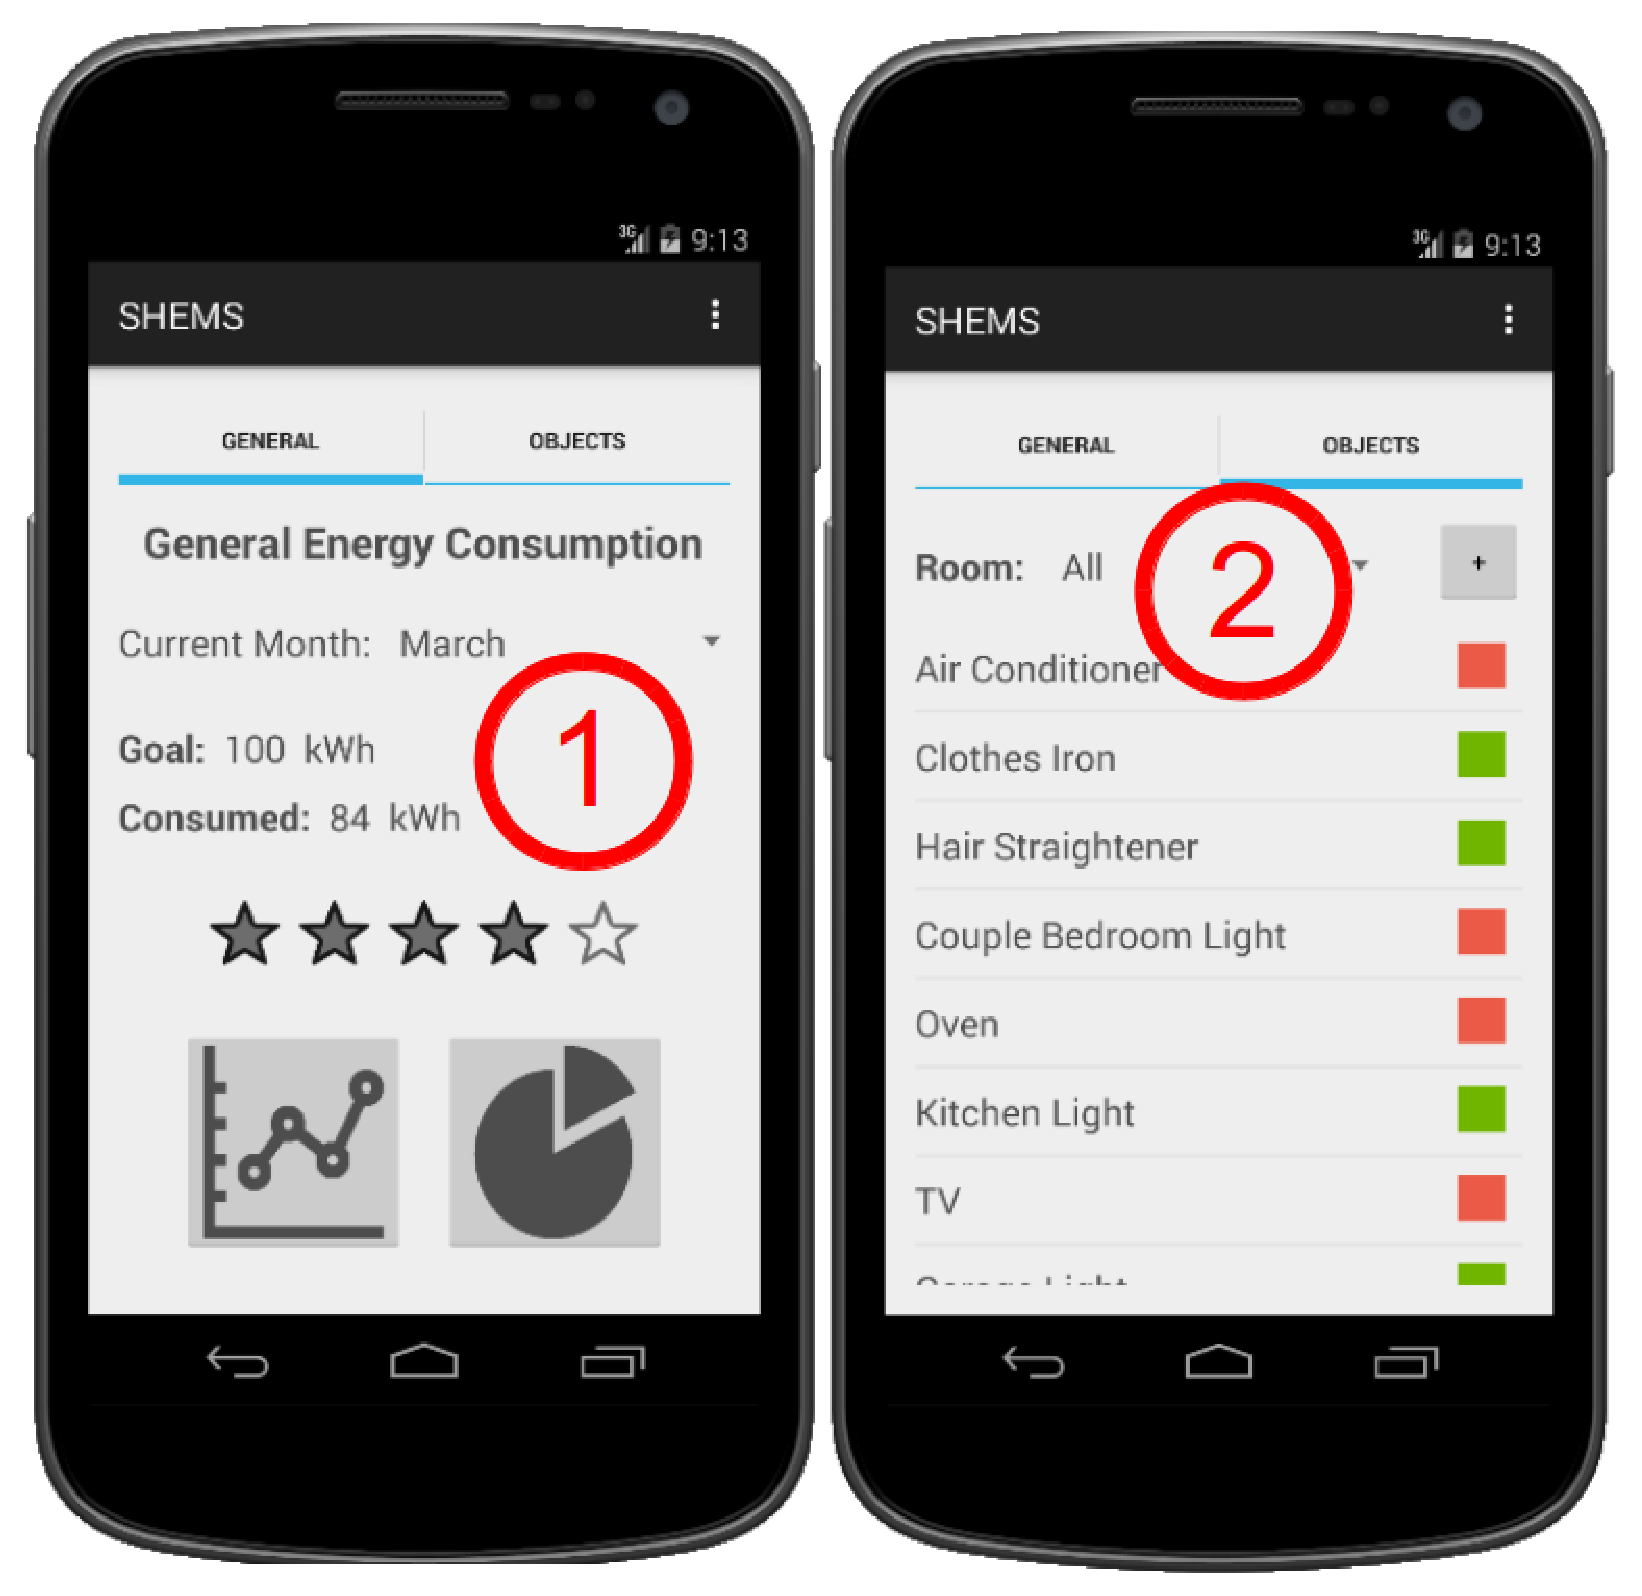
\includegraphics[width=\marginparwidth]{images/mobile_goal-filter.eps}
  \caption{Mobile version. Number 1 represents the \textbf{goal} feature and number 2 represents the \textbf{filter} feature.}
  \label{fig:mobileprint}
  \end{center}  
\end{figure}

\begin{figure}
  \begin{center}
  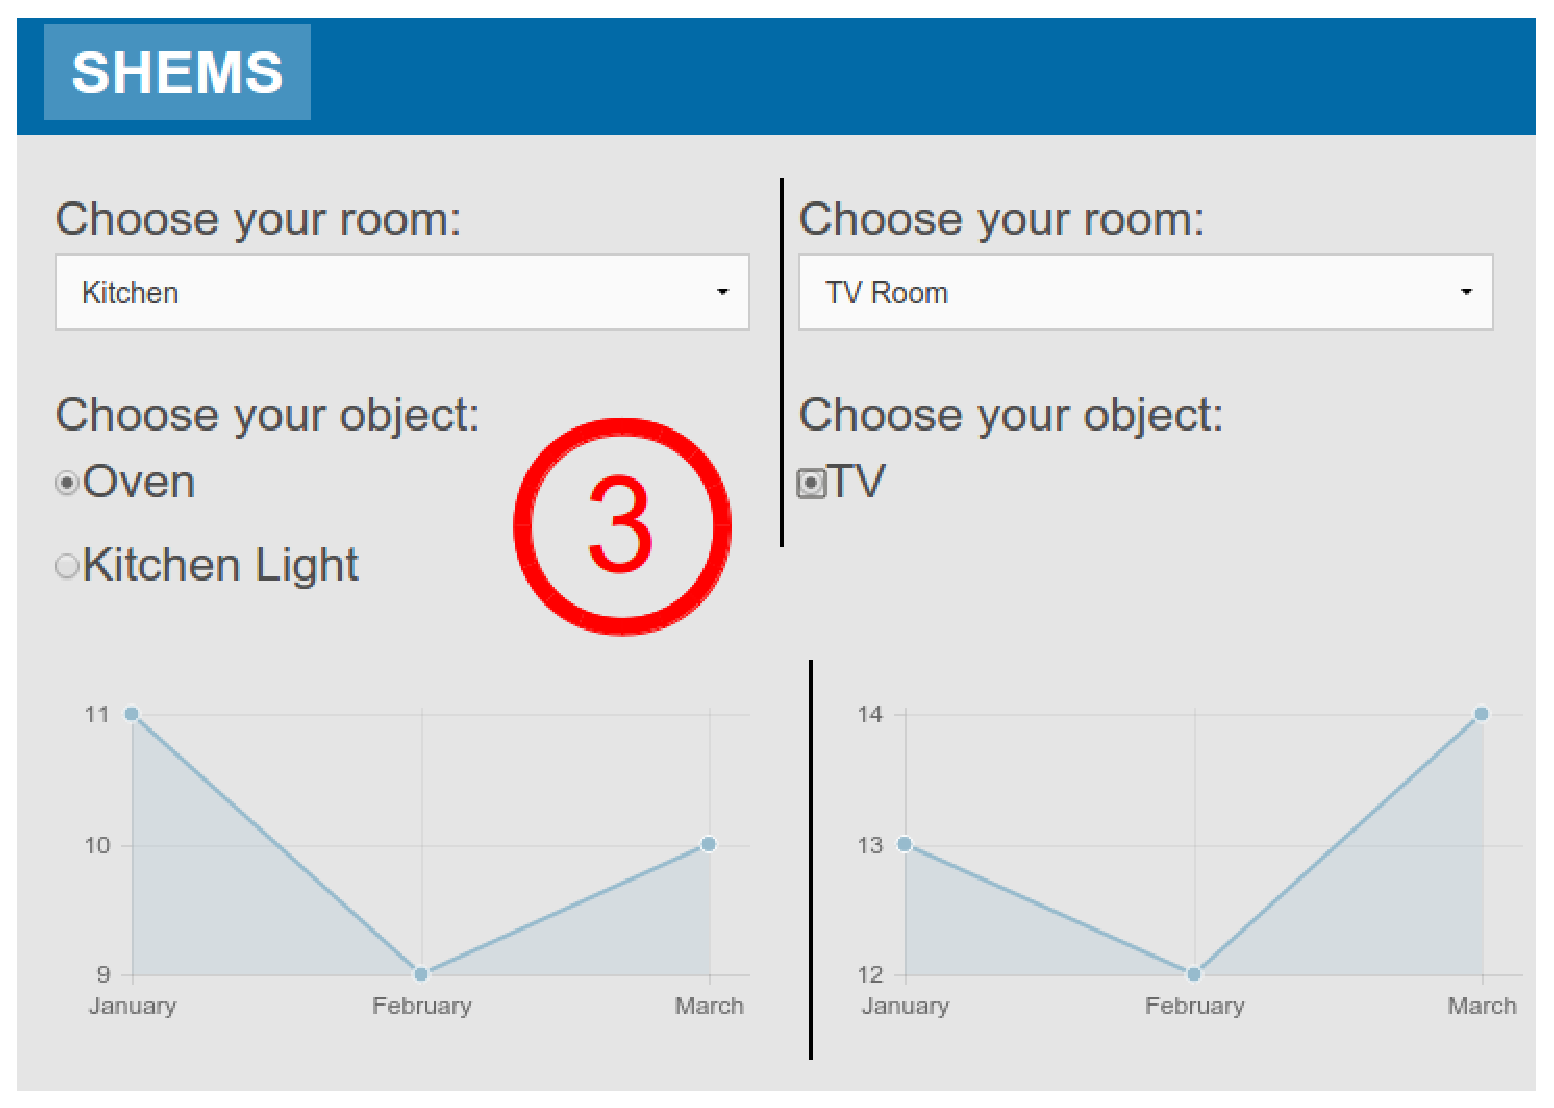
\includegraphics[width=\marginparwidth]{images/web1_comparator.eps}
  \caption{Other web version. Number 3 represents the \textbf{comparator} feature.}
  \label{fig:web1print}
  \end{center}  
\end{figure}
}

Another interesting approach, proposed in~\cite{test-image-comparison-korea}, uses the idea of record and playblack with the automation of the analysis of the results through image comparison. In this solution, after the execution of a test script, the image of the UI is recorded. It can be used later to verify if changes in the system affected the UI, comparing automatically the old and new images of the UI.
 
Another related work, presented in~\cite{ui-equilavance-raquel}, is not strictly about testing, but comparing UIs of the same system that are adapted to different contexts. In this approach, the UIs are abstracted to formal models based on graphs and the abstractions can be automatically compared, verifying if  they have the same capabilities and appearance.

% =============================================================================
\section{Case Study}
% =============================================================================

The case study used in this work is a prototype for a smart home energy management system. This decision is based on the fact that it is a modern concept, little explored in the domain of this research and whose UIs can be adapted to several contexts. A smart home may be defined as a well-designed structure with sufficient access to assets, communication, controls, data, and information technologies for enhancing the occupants' quality of life through comfort, convenience, reduced costs and increased connectivity~\cite{smart-home-harper}. A smart home energy management system is an energy management system applied to smart homes. It allows users to control and monitor the energy consumption in a residence from different devices. 

It is a prototype because we have developed only the UIs of the system for four versions, three for web environment and one as a mobile application. The data of the system are predetermined. All versions have the same features, except for two web versions that have an additional feature. The differences between the versions are visual. In the case of the mobile application, the UI is adapted to a mobile device, which contains a smaller screen and its own platform for UI development. In the case of the web versions, the UIs have also been developed to this context, using web UI technologies. But the differences between the three web versions are changes in the navigation and UI components. In this paper, we focus on the following features of the prototype:

\begin{enumerate}
\item \textbf{Goal}: the user can check information about the general energy consumption per month. Having access to the goal and consumption in kWh for the chosen month. See \autoref{fig:web0print} and \autoref{fig:mobileprint}.

\item \textbf{Filter}: the user has access to a list of all his or her objects in the house, having the possibility to filter this list per room. An object means any component that can be controlled and whose energy consumption can be registered, such as lights and electronic devices. See \autoref{fig:web0print} and \autoref{fig:mobileprint}.

\item \textbf{Comparator}: the user can choose two objects and compare, side by side, their energy consumption charts. This feature is present in only two of the web versions. See \autoref{fig:web1print}
\end{enumerate} 

The purpose is to test each feature using execution automation tools for UI testing. For instance Selenium~\cite{selenium} for the web versions and Selendroid~\cite{selendroid} for the mobile version. The approach to test the \textbf{goal} feature is to make these tools to change the current month, interacting with the combobox filter component, and then to verify if the goal and consumed labels have the right value. In the case of the \textbf{filter} feature, the tools have to interact with the filter, changing the current room and verifying if the only correct objects are displayed in the screen. Finally, the \textbf{compator} feature can be tested by using the tools to change the room filter, to chose the objects using the checkbox and to verify if the charts are displayed.


% =============================================================================
\section{Approach: generating test scripts for UI testing from abstract descriptions}
% =========================================
\subsection{Principle}
TODO

\subsection{Principles put into Practice}
TODO

\subsection{Discussion and Analysis}
Firstly, the number of lines to write for tests have been at least halved, as Table \ref{table:scriptssize} shows it.
\begin{table}
\begin{tabular}{l l r r r r}
			&					&	mobile	&	web0	&	web1	&	web2	\\
goal		&	plain Java	&	161		&	143		&	151		&	147		\\
			&	with Tobias	&	76		&	67		&	69		&	68		\\
filter		&	plain Java	&	/		&	350		&	402		&	369		\\
			&	with Tobias	&	/		&	88		&	93		&	92		\\
compare	&	plain Java	&	/		&	/		&	235		&	227		\\
			&	with Tobias	&	/		&	/		&	59		&	58
\end{tabular}
\caption{Comparison of number of lines for various functionalities and various versions for Tobias script and its generated test}
\label{table:scriptssize}
\end{table}
Secondly, the logical structure of the various tests for a same functionality and version is shared, and so the differences between these files are very localized : in the header of the file (preferences for the test) and in the implementations of the abstract groups (version details). So there is little variation from a shared abstract script for each file, as can be seen in Table \ref{table:scripts-similarity}.
\begin{table}
\begin{tabular}{l l r r r}
			&			&	shared	&	total	&	\%	\\
goal		&	mobile	&	48		&	76		&	63	\\
			&	web0	&	65		&	67		&	97	\\
			&	web2	&	65		&	68		&	95	\\
filter		&	web0	&	78		&	88		&	88	\\
			&	web2	&	89		&	92		&	96	\\
compare	&	web2	&	55		&	58		&	94
\end{tabular}
\caption{Comparison of number of shared lines between Tobias scripts and version web1 for a same functionality}
\label{table:scripts-similarity}
\end{table}
When small changes are applied to the UI, the scripts only differ by some lines. Even in the case of a change of platform (web to mobile) the scripts stay similar.
Lastly, there is also shared lines between files, whichever their version and functionality tested, because these tests proceed by steps, which can sometimes be the same for several scripts.
So this approach allows to reduce the amount of work, while it facilitates it by reducing differences between script versions.

% =============================================================================
\section{Conclusions and Perspectives}
% =============================================================================
Because of the similarities, these scripts could easily be generated from a single script, containing the abstract test cases and the implementation details. Tobias could do it if its entry language syntax (TSLT) would be improved.
TODO

\balance
\bibliographystyle{acm-sigchi}
\bibliography{ref}

\end{document}